\documentclass[12pt]{../../oss-apphys-exam}
\usepackage{enumitem}

\usetikzlibrary{patterns}

\tikzset{
  >=latex
}
\setlength\extrarowheight{5pt}
\renewcommand{\arraystretch}{1.7}

\runningheader{
  \fontfamily{phv}\small
  \textcolor{gray}{AP PHYSICS C: MECHANICS $\blacksquare$}
  \textbf{FREE-RESPONSE QUESTIONS}}{}{}


\begin{document}

\begin{center}
  {
    \fontfamily{phv}\Large
    \textbf{PHYSICS C: MECHANICS\\SECTION II\\TIME -- 60 MINUTES}
  }
\end{center}

\vspace{2in}
\textbf{Directions:}

Section II has 3 questions and lasts 60 minutes.

You may use the available paper for scratch work and planning, but you must
write your answers in the free-response booklet. Label parts (e.g., \textbf{A},
\textbf{B}, \textbf{C}) and sub-parts (e.g., i, ii, iii) as needed. Use a
pencil or a pen with black or dark blue ink to write your responses.

A calculator is allowed in this section, as well as a ruler and straightedge.
You may use a handheld four-function, scientific, or graphing calculator, or
the calculator available in this application. Reference information, including
lists of equations, can also be accessed in this application and is available
throughout the exam.

All final numerical answers should include appropriate units when applicable.
Credit for your work depends on demonstrating that you know which physical
principles to apply in a particular situation. Credit will be awarded only for
work that is clearly designated as the solution to a specific part of a
question. Credit also depends on the quality of your solutions and explanations.
Therefore, you should show your work for each part in the space provided for
that part. If you need more space, be sure to clearly indicate where you
continue your work. When constructing a graph or diagram, use only one color of
ink or pencil.

You may pace yourself as you answer the questions in this section, or you may
use these optional timing recommendations:

It is suggested that you spend about 20 minutes on each question.

You can go back and forth between questions in this section until time expires.
The clock will turn red when 5 minutes remain---\textbf{the proctor will not
  give you any time updates or warnings.}
\newpage


% THIS QUESTION IS BASED ON THE 2023 AP PHYSICS C MECHANICS EXAM SET 2
% QUESTION 1. FOR NOW, IT IS USED WITHOUT MODIFICATIONS

\begin{center}
  \pic{.6}{vertical-springs}
\end{center}

\begin{questions}
  \question A student conducts an investigation to determine the relationship
  between the period of oscillation $T$ of a system consisting of a block and
  $N$ attached springs. The student starts with a block of mass $m$ attached
  to a single ideal spring of spring constant $k$, as shown in Figure 1. The
  student holds the block so that the spring is neither stretched nor
  compressed at a vertical height \SI{1.00}{\metre} above a motion detector.
  The student releases the block from rest and records the period of
  oscillation for the system consisting of the single spring and block. An
  additional identical spring is attached in parallel, as shown in Figure 2,
  and the procedure is repeated for $N=2$ springs. This procedure is repeated
  through $N=10$ springs.

  \begin{parts}
    \part\textbf{Derive} an expression for $T$ as a function of $N$. Express
    your answer in terms of $m$, $k$, $N$, and physical constants as
    appropriate.

    \part On the following axes, \textbf{sketch} a graph of $T$ as a function
    of $N$ for $N\geq1$.
    \begin{center}
      \begin{tikzpicture}[scale=.8]
        \draw[axes] (0,0)--(8,0) node[right]{$N$};
        \draw[axes] (0,0)--(0,5.5) node[above]{$T$};
      \end{tikzpicture}
    \end{center}
    \newpage
    \uplevel{
      The student plots the data for $T^2$ as a function of $N^{-1}$, as shown.
      \begin{center}
        \pic{.7}{data-points}
      \end{center}
    }


    \part\textbf{Draw} the best-fit line for the data.\label{best}
    
    \part The mass of the block is measured to be $m=\SI{1.5}{\kilo\gram}$.
    Using the graph, \textbf{calculate} an experimental value for the spring
    constant $k$ for a single spring.
    
    \part The student finds that the value given by the manufacturer for the
    spring constant is larger than the value determined experimentally in part
    \textbf{D}. Determine a single source of experimental error that could
    result in the observed difference in the value for $k$. Briefly
    \textbf{justify} your answer.
    \newpage
    
    \uplevel{
      \begin{center}
        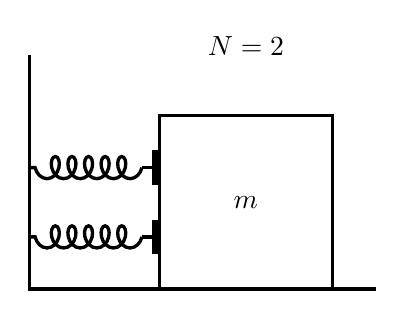
\begin{tikzpicture}[very thick,scale=1.1]
          \draw (2.5,0)--(-1.5,0)--(-1.5,2.7);
          \draw rectangle (2,2) node[midway]{$m$};
          \fill (-.08,.8) rectangle (0,.4);
          \fill (-.08,1.2) rectangle (0,1.6);

          \draw (0,.6)--(-.2,.6);
          \draw[
            decoration={aspect=.7,segment length=6,amplitude=4,coil},
            decorate] (-.2,.6)--(-1.5,.6);

          \draw (0,1.4)--(-.2,1.4);
          \draw[
            decoration={aspect=.7,segment length=6,amplitude=4,coil},
            decorate] (-.2,1.4)--(-1.5,1.4);

          \node at (1,2.8) {$N=2$};
        \end{tikzpicture}\\
        Figure 3
      \end{center}
      The student conducts a similar investigation to determine the
      relationship between the period of oscillation $T$ of a system consisting
      of a block and a number $N$ of identical springs but arranges the
      block-spring system horizontally on a table, as shown in Figure 3.
      Frictional forces between the table and the block are negligible. In each
      trial, the block is displaced the same horizontal distance from
      equilibrium and released from rest.
    }
    
    \part The student plots $T^2$ as a function of $N^{-1}$ for this new data.
    Would the slope of the best-fit line from this new investigation be greater
    than, less than, or the same as the slope of the best-fit line in part
    \textbf{C}? \textbf{Justify} your answer.

    \vspace{.2in}
    \underline{\hspace{.5in}} greater than \hspace{.5in}
    \underline{\hspace{.5in}} less than \hspace{.5in}
    \underline{\hspace{.5in}} the same as
    
    \part When $N=1$, the maximum speed of the block is found to be
    $v_\text{max}$. When $N$ increases, will $v_\text{max}$ increase, decrease,
    or stay the same? \textbf{Justify} your answer.

    \vspace{.2in}
    \underline{\hspace{.5in}} increase \hspace{.5in}
    \underline{\hspace{.5in}} decrease \hspace{.5in}
    \underline{\hspace{.5in}} stay the same
    \end{parts}
  \newpage

  % THIS QUESTION IS BASED ON THE 2019 AP PHYSICS C MECHANICS PRACTICE TEST
  % QUESTION 3.
  
  \uplevel{
    \centering
    \pic{.55}{pulley-mass}
  }
  
  \question Three blocks are connected by strings that pass over pulleys of
  negligible mass. Block  is on a level, horizontal surface of negligible
  friction. Block A is on top of block B. String 1 connects blocks A and B. The
  coefficients of static and kinetic friction between blocks A and B are
  $\mu_s$ and $\mu_k$, respectively. Block C is hanging over the end of the
  table and is attached to block B by string 2, as shown above. The masses of
  blocks A, B, and C are $m_A$, $m_B$, and $m_C$, respectively. When block C is
  released, the system remains at rest.
  \begin{parts}
    \part On the dot below, which represents block A, \textbf{draw and label}
    the forces (not components) that act on block A. Each force must be
    represented by a distinct arrow starting on, and pointing away from, the
    dot.
    \begin{center}
      \underline{Block A}

      \vspace{.6in}{\tikz\fill circle(.15);}\vspace{.6in}
    \end{center}

    \part On the dot below, which represents block B, \textbf{draw and label}
    the forces (not components) that act on block B. Each force must be
    represented by a distinct arrow starting on, and pointing away from, the
    dot.
    \begin{center}
      \underline{Block B}

      \vspace{.6in}{\tikz\fill circle(.15);}\vspace{.6in}
    \end{center}

    \part Derive an expression for the maximum value for $m_C$ at which the
    blocks will remain at rest. Express all algebraic answers in terms of
    $\mu_s$, $\mu_k$, $m_A$, $m_B$, $m_C$, and physical constants, as
    appropriate.
    \vspace{\stretch1}
    \newpage
    \uplevel{
      \begin{center}
        \pic{.53}{clay}
      \end{center}
      The setup is modified, as shown in the figure above. Block A and one of
      the pulleys are removed, and block B remains on the table. There is still
      negligible friction between block B and the table. A lump of clay is
      added to block B. The students use second law of motion to derive an
      equation for the acceleration $a_C$ of block C. The acceleration is given
      by the equation
      \begin{displaymath}
        a_C=\frac{m_C}{m_\text{tot}}g
      \end{displaymath}
      where $m_\text{tot}$ is the combined mass of the clay and the two blocks.
      Students use the setup shown above to experimentally determine the
      acceleration $g$ due to gravity. In each trial, a student moves a small
      amount of clay from block B to block C and then releases the blocks from
      rest, recording the new values of $m_C$ and $a_C$. The total mass of the
      clay and the two blocks is $m_\text{tot}=\SI{5.0}{\kilo\gram}$. The graph
      below shows $a_C$ as a function of $m_C$ , where $m_C$ is now the
      combined mass of block C and the mass of clay added to block C.
      
      \begin{center}
        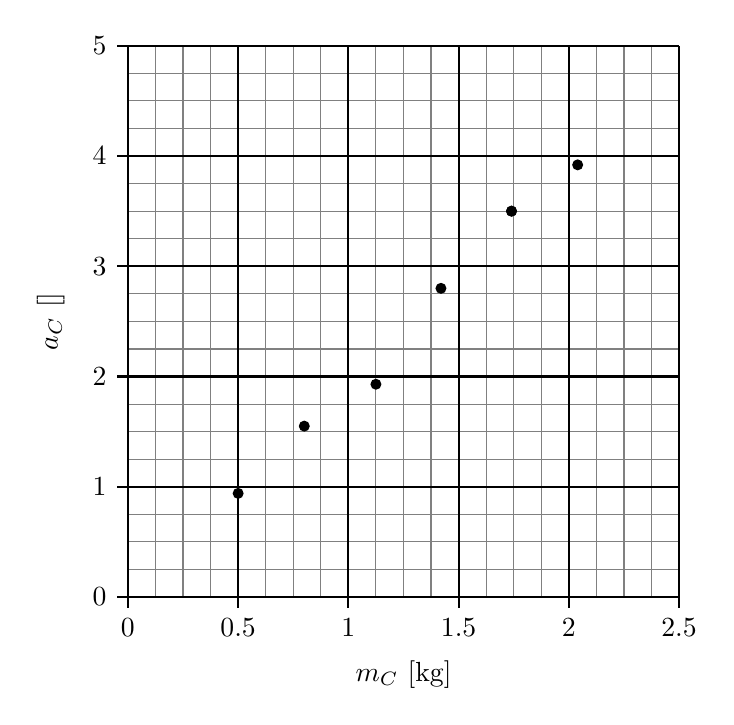
\begin{tikzpicture}[scale=1.4]
          \draw[gray, step=.25] grid (5,5);
          \draw[thick] grid (5,5);
          \foreach \y in {0,...,5}
          \draw[thick] (0,\y)--+(-.1,0) node[left]{$\y$};
          \foreach \x in {0,0.5,...,2.5}
          \draw[thick] (\x*2,0)--+(0,-.1) node[below]{$\x$};

          \node at (2.5,-.7) {$m_C$ [kg]};
          \node[rotate=90] at (-.7,2.5){
            $a_C$ [\si{\metre\per\second\squared}]};
          \fill (1,.94) circle (.05);
          \fill (1.6,1.55) circle (.05);
          \fill (2.25,1.93) circle (.05);
          \fill (2.84,2.8) circle (.05);
          \fill (3.48,3.5) circle (.05);
          \fill (3.48,3.5) circle (.05);
          \fill (4.08,3.92) circle (.05);
        \end{tikzpicture}
      \end{center}
    }
      
    \part\textbf{Draw} a best-fit line to the data points in the graph above.
    \label{best-fit-again}
    
    \part Use the best-fit line from part \textbf{D} to \textbf{calculate} an
    experimental value for the acceleration $g$ due to gravity
    
    \part If the mass of the pulley in part \textbf{D} is significant, would
    the experimental value of $g$ be greater than, less than, or equal to the
    value calculated in part \textbf{E}? \textbf{Justify} your answer.

    \vspace{.2in}
    \underline{\hspace{.5in}} Greater than \hspace{.5in}
    \underline{\hspace{.5in}} Less than \hspace{.5in}
    \underline{\hspace{.5in}} Equal to
    \newpage
    
    \part A different group of students repeats the experiment, but instead of
    moving clay from block B to block C, they just remove a small amount of
    clay from block B and set it aside, away from the setup. The equation
    $a_C=m_C g/ m_\text{tot}$ still applies to the new experiment. In order to
    provide a straight-line graph that can be used to determine an
    experimental value for $g$, what two quantities should the students now
    graph? Check all that apply. \textbf{Justify} your answer.

    \vspace{.2in}
    \begin{tabular}{lll}
      \underline{\hspace{.4in}} $a_c$ VS.\ $\dfrac1{m_\text{tot}}$ \hspace{.5in}&
      \underline{\hspace{.4in}} $a_c$ VS.\ $m_\text{tot}$ \hspace{.5in} &
      \underline{\hspace{.4in}} $a_c$ VS.\ $\dfrac{m_C}{m_\text{tot}}$ \\

      \underline{\hspace{.4in}} $a_c$ VS.\ $m_C$  \hspace{.5in} &
      \underline{\hspace{.4in}} $m_C$ VS.\ $m_\text{tot}$ \hspace{.5in} &
      \underline{\hspace{.4in}} $m_C$ VS.\ $\dfrac1{m_\text{tot}}$ \\
    \end{tabular}
  \end{parts}
  \newpage
  
  % THIS QUESTION IS A SLIGHTLY MODIFIED VERSION OF THE 2008 AP PHYSICS C
  % MECHANICS EXAM PRACTICE TEST QUESTION 1. IT HAS BEEN MODIFIED TO REFLECT
  % THE LANGUAGE USED IN MORE CURRENT AP EXAMS.
  
  \uplevel{
    \cpic{.35}{spool}
  }
  \question A student holds one end of a thread, which is wrapped around a
  cylindrical spool, as shown above. The student then drops the spool from a
  height $h$ above the floor, and the thread unwinds as it falls. The spool has
  a mass $M$ and a radius R, and the thread has negligible mass. The spool can
  be approximated as a solid cylinder with rotational moment $I=\dfrac12MR^2$.
  Express your answers in terms of $M$, $R$, $h$, and fundamental constants.
  \begin{parts}
    \part\textbf{Derive} an expression for the magnitude of linear acceleration
    ($a$) of the spool as it falls.

    \part\textbf{Derive} an expression for the magnitude of the angular
    velocity ($\omega$) of the spool just before it strikes the floor.
    
    \uplevel{
      At time $t=0$, the spinning spool lands on the floor without bouncing and
      comes free from the thread. It continues to spin, but slips on the
      floor's surface while doing so. Assume a constant coefficient of sliding
      friction $\mu$.
    }

    \part\textbf{Derive} an algebraic expression for the angular velocity
    ($\omega$) of the spool as a function of time $t$.
    
    \part\textbf{Derive} an algebraic expression for the horizontal speed ($v$)
    of the spool as a function of time, assuming the horizontal speed is zero at
    time $t=0$.
    
    \part\textbf{Calculate} the time $T$ when slipping between the spool and
    floor cease?
  \end{parts}
\end{questions}
\end{document}
